\documentclass[onecolumn, draftclsnofoot,10pt, compsoc]{IEEEtran}

\usepackage{graphicx}                                        
\usepackage{amssymb}                                         
\usepackage{amsmath}                                         
\usepackage{amsthm}                                          
\usepackage{alltt}                                           
\usepackage{float}
\usepackage{color}
\usepackage{url}
\usepackage{balance}
\usepackage[TABBOTCAP, tight]{subfigure}
\usepackage{enumitem}
\usepackage{pstricks, pst-node}
\usepackage[T1]{fontenc}
\graphicspath{{images/}}
\usepackage{caption}

\usepackage{geometry}
\geometry{letterpaper, margin=0.75in}

\newcommand{\cred}[1]{{\color{red}#1}}
\newcommand{\cblue}[1]{{\color{blue}#1}}
\newcommand{\toc}{\tableofcontents}
\newlength{\drop}

\def\name{Mark Bereza}

\usepackage{fancyvrb}
\usepackage{color}
\usepackage[latin1]{inputenc}


\makeatletter
\def\PY@reset{\let\PY@it=\relax \let\PY@bf=\relax%
    \let\PY@ul=\relax \let\PY@tc=\relax%
    \let\PY@bc=\relax \let\PY@ff=\relax}
\def\PY@tok#1{\csname PY@tok@#1\endcsname}
\def\PY@toks#1+{\ifx\relax#1\empty\else%
    \PY@tok{#1}\expandafter\PY@toks\fi}
\def\PY@do#1{\PY@bc{\PY@tc{\PY@ul{%
    \PY@it{\PY@bf{\PY@ff{#1}}}}}}}
\def\PY#1#2{\PY@reset\PY@toks#1+\relax+\PY@do{#2}}

\expandafter\def\csname PY@tok@gd\endcsname{\def\PY@tc##1{\textcolor[rgb]{0.63,0.00,0.00}{##1}}}
\expandafter\def\csname PY@tok@gu\endcsname{\let\PY@bf=\textbf\def\PY@tc##1{\textcolor[rgb]{0.50,0.00,0.50}{##1}}}
\expandafter\def\csname PY@tok@gt\endcsname{\def\PY@tc##1{\textcolor[rgb]{0.00,0.25,0.82}{##1}}}
\expandafter\def\csname PY@tok@gs\endcsname{\let\PY@bf=\textbf}
\expandafter\def\csname PY@tok@gr\endcsname{\def\PY@tc##1{\textcolor[rgb]{1.00,0.00,0.00}{##1}}}
\expandafter\def\csname PY@tok@cm\endcsname{\let\PY@it=\textit\def\PY@tc##1{\textcolor[rgb]{0.25,0.50,0.50}{##1}}}
\expandafter\def\csname PY@tok@vg\endcsname{\def\PY@tc##1{\textcolor[rgb]{0.10,0.09,0.49}{##1}}}
\expandafter\def\csname PY@tok@m\endcsname{\def\PY@tc##1{\textcolor[rgb]{0.40,0.40,0.40}{##1}}}
\expandafter\def\csname PY@tok@mh\endcsname{\def\PY@tc##1{\textcolor[rgb]{0.40,0.40,0.40}{##1}}}
\expandafter\def\csname PY@tok@go\endcsname{\def\PY@tc##1{\textcolor[rgb]{0.50,0.50,0.50}{##1}}}
\expandafter\def\csname PY@tok@ge\endcsname{\let\PY@it=\textit}
\expandafter\def\csname PY@tok@vc\endcsname{\def\PY@tc##1{\textcolor[rgb]{0.10,0.09,0.49}{##1}}}
\expandafter\def\csname PY@tok@il\endcsname{\def\PY@tc##1{\textcolor[rgb]{0.40,0.40,0.40}{##1}}}
\expandafter\def\csname PY@tok@cs\endcsname{\let\PY@it=\textit\def\PY@tc##1{\textcolor[rgb]{0.25,0.50,0.50}{##1}}}
\expandafter\def\csname PY@tok@cp\endcsname{\def\PY@tc##1{\textcolor[rgb]{0.74,0.48,0.00}{##1}}}
\expandafter\def\csname PY@tok@gi\endcsname{\def\PY@tc##1{\textcolor[rgb]{0.00,0.63,0.00}{##1}}}
\expandafter\def\csname PY@tok@gh\endcsname{\let\PY@bf=\textbf\def\PY@tc##1{\textcolor[rgb]{0.00,0.00,0.50}{##1}}}
\expandafter\def\csname PY@tok@ni\endcsname{\let\PY@bf=\textbf\def\PY@tc##1{\textcolor[rgb]{0.60,0.60,0.60}{##1}}}
\expandafter\def\csname PY@tok@nl\endcsname{\def\PY@tc##1{\textcolor[rgb]{0.63,0.63,0.00}{##1}}}
\expandafter\def\csname PY@tok@nn\endcsname{\let\PY@bf=\textbf\def\PY@tc##1{\textcolor[rgb]{0.00,0.00,1.00}{##1}}}
\expandafter\def\csname PY@tok@no\endcsname{\def\PY@tc##1{\textcolor[rgb]{0.53,0.00,0.00}{##1}}}
\expandafter\def\csname PY@tok@na\endcsname{\def\PY@tc##1{\textcolor[rgb]{0.49,0.56,0.16}{##1}}}
\expandafter\def\csname PY@tok@nb\endcsname{\def\PY@tc##1{\textcolor[rgb]{0.00,0.50,0.00}{##1}}}
\expandafter\def\csname PY@tok@nc\endcsname{\let\PY@bf=\textbf\def\PY@tc##1{\textcolor[rgb]{0.00,0.00,1.00}{##1}}}
\expandafter\def\csname PY@tok@nd\endcsname{\def\PY@tc##1{\textcolor[rgb]{0.67,0.13,1.00}{##1}}}
\expandafter\def\csname PY@tok@ne\endcsname{\let\PY@bf=\textbf\def\PY@tc##1{\textcolor[rgb]{0.82,0.25,0.23}{##1}}}
\expandafter\def\csname PY@tok@nf\endcsname{\def\PY@tc##1{\textcolor[rgb]{0.00,0.00,1.00}{##1}}}
\expandafter\def\csname PY@tok@si\endcsname{\let\PY@bf=\textbf\def\PY@tc##1{\textcolor[rgb]{0.73,0.40,0.53}{##1}}}
\expandafter\def\csname PY@tok@s2\endcsname{\def\PY@tc##1{\textcolor[rgb]{0.73,0.13,0.13}{##1}}}
\expandafter\def\csname PY@tok@vi\endcsname{\def\PY@tc##1{\textcolor[rgb]{0.10,0.09,0.49}{##1}}}
\expandafter\def\csname PY@tok@nt\endcsname{\let\PY@bf=\textbf\def\PY@tc##1{\textcolor[rgb]{0.00,0.50,0.00}{##1}}}
\expandafter\def\csname PY@tok@nv\endcsname{\def\PY@tc##1{\textcolor[rgb]{0.10,0.09,0.49}{##1}}}
\expandafter\def\csname PY@tok@s1\endcsname{\def\PY@tc##1{\textcolor[rgb]{0.73,0.13,0.13}{##1}}}
\expandafter\def\csname PY@tok@sh\endcsname{\def\PY@tc##1{\textcolor[rgb]{0.73,0.13,0.13}{##1}}}
\expandafter\def\csname PY@tok@sc\endcsname{\def\PY@tc##1{\textcolor[rgb]{0.73,0.13,0.13}{##1}}}
\expandafter\def\csname PY@tok@sx\endcsname{\def\PY@tc##1{\textcolor[rgb]{0.00,0.50,0.00}{##1}}}
\expandafter\def\csname PY@tok@bp\endcsname{\def\PY@tc##1{\textcolor[rgb]{0.00,0.50,0.00}{##1}}}
\expandafter\def\csname PY@tok@c1\endcsname{\let\PY@it=\textit\def\PY@tc##1{\textcolor[rgb]{0.25,0.50,0.50}{##1}}}
\expandafter\def\csname PY@tok@kc\endcsname{\let\PY@bf=\textbf\def\PY@tc##1{\textcolor[rgb]{0.00,0.50,0.00}{##1}}}
\expandafter\def\csname PY@tok@c\endcsname{\let\PY@it=\textit\def\PY@tc##1{\textcolor[rgb]{0.25,0.50,0.50}{##1}}}
\expandafter\def\csname PY@tok@mf\endcsname{\def\PY@tc##1{\textcolor[rgb]{0.40,0.40,0.40}{##1}}}
\expandafter\def\csname PY@tok@err\endcsname{\def\PY@bc##1{\setlength{\fboxsep}{0pt}\fcolorbox[rgb]{1.00,0.00,0.00}{1,1,1}{\strut ##1}}}
\expandafter\def\csname PY@tok@kd\endcsname{\let\PY@bf=\textbf\def\PY@tc##1{\textcolor[rgb]{0.00,0.50,0.00}{##1}}}
\expandafter\def\csname PY@tok@ss\endcsname{\def\PY@tc##1{\textcolor[rgb]{0.10,0.09,0.49}{##1}}}
\expandafter\def\csname PY@tok@sr\endcsname{\def\PY@tc##1{\textcolor[rgb]{0.73,0.40,0.53}{##1}}}
\expandafter\def\csname PY@tok@mo\endcsname{\def\PY@tc##1{\textcolor[rgb]{0.40,0.40,0.40}{##1}}}
\expandafter\def\csname PY@tok@kn\endcsname{\let\PY@bf=\textbf\def\PY@tc##1{\textcolor[rgb]{0.00,0.50,0.00}{##1}}}
\expandafter\def\csname PY@tok@mi\endcsname{\def\PY@tc##1{\textcolor[rgb]{0.40,0.40,0.40}{##1}}}
\expandafter\def\csname PY@tok@gp\endcsname{\let\PY@bf=\textbf\def\PY@tc##1{\textcolor[rgb]{0.00,0.00,0.50}{##1}}}
\expandafter\def\csname PY@tok@o\endcsname{\def\PY@tc##1{\textcolor[rgb]{0.40,0.40,0.40}{##1}}}
\expandafter\def\csname PY@tok@kr\endcsname{\let\PY@bf=\textbf\def\PY@tc##1{\textcolor[rgb]{0.00,0.50,0.00}{##1}}}
\expandafter\def\csname PY@tok@s\endcsname{\def\PY@tc##1{\textcolor[rgb]{0.73,0.13,0.13}{##1}}}
\expandafter\def\csname PY@tok@kp\endcsname{\def\PY@tc##1{\textcolor[rgb]{0.00,0.50,0.00}{##1}}}
\expandafter\def\csname PY@tok@w\endcsname{\def\PY@tc##1{\textcolor[rgb]{0.73,0.73,0.73}{##1}}}
\expandafter\def\csname PY@tok@kt\endcsname{\def\PY@tc##1{\textcolor[rgb]{0.69,0.00,0.25}{##1}}}
\expandafter\def\csname PY@tok@ow\endcsname{\let\PY@bf=\textbf\def\PY@tc##1{\textcolor[rgb]{0.67,0.13,1.00}{##1}}}
\expandafter\def\csname PY@tok@sb\endcsname{\def\PY@tc##1{\textcolor[rgb]{0.73,0.13,0.13}{##1}}}
\expandafter\def\csname PY@tok@k\endcsname{\let\PY@bf=\textbf\def\PY@tc##1{\textcolor[rgb]{0.00,0.50,0.00}{##1}}}
\expandafter\def\csname PY@tok@se\endcsname{\let\PY@bf=\textbf\def\PY@tc##1{\textcolor[rgb]{0.73,0.40,0.13}{##1}}}
\expandafter\def\csname PY@tok@sd\endcsname{\let\PY@it=\textit\def\PY@tc##1{\textcolor[rgb]{0.73,0.13,0.13}{##1}}}

\def\PYZbs{\char`\\}
\def\PYZus{\char`\_}
\def\PYZob{\char`\{}
\def\PYZcb{\char`\}}
\def\PYZca{\char`\^}
\def\PYZam{\char`\&}
\def\PYZlt{\char`\<}
\def\PYZgt{\char`\>}
\def\PYZsh{\char`\#}
\def\PYZpc{\char`\%}
\def\PYZdl{\char`\$}
\def\PYZti{\char`\~}
% for compatibility with earlier versions
\def\PYZat{@}
\def\PYZlb{[}
\def\PYZrb{]}
\makeatother


\parindent = 0.0 in
\parskip = 0.1 in

\begin{document}

\begin{titlepage}
\begin{center}

\vspace*{50mm}

\textsc{\LARGE CS444: Operating Systems II}\\[1.5cm]

\hrule
\vspace{5mm}
{ \huge \bfseries Processes, Threads, and CPU Scheduling \\[0.9cm] }
\hrule 
\vspace{5mm}

\noindent
\begin{minipage}{0.4\textwidth}

\begin{flushleft} \large
\emph{Author:}\\
Mark \textsc{Bereza}
\end{flushleft}
\end{minipage}%
\begin{minipage}{0.4\textwidth}
\begin{flushright} \large
\emph{Instructor:} \\
D. Kevin \textsc{McGrath}
\end{flushright}

\end{minipage}

\vspace*{\fill}
{\large \today}\\
{\large Fall Term}

\end{center}
\end{titlepage}
  
\tableofcontents
\newpage

\section{Introduction}
Since the modern personal computer has become an all-purpose computation tool, it is critical that it is able to run multiple programs simultaneously (either concurrently through the use of multiple cores or with the illusion of concurrency accomplished through a combination of time sharing and scheduling). As a result, operating systems have been created and improved upon primarily to address this challenge - the creation, destruction, resource management, and scheduling of multiple executing programs, or processes. While support for these basic responsibilities is ubiquitous in most modern operating systems, the actual implementation of concepts such as processes, threads, and CPU scheduling can vary greatly from OS to OS. This paper in particular will look at how FreeBSD's and Windows' implementations of these concepts compare to Linux.
\section{Processes and Threads}
A process, in its simplest terms, is an instance of an executing program. Usually processes have access to their own set of virtual memory independent of other processes. A thread, on the other hand, is a more granular worker employed by a process to actually perform its work. It is not uncommon for a single process to spawn and manage many threads, each sharing some common process resources to accomplish a larger common task.

In Windows, although the high-level implementation of processes and threads is fairly straight-forward, the data structures describing them and the steps needed to initialize them are extremely complex. Each process is described using an EPROCESS structure associated with at least one ETHREAD structure \cite{WindowsInternals}. Processes are created using the CreateProcess() system call, which copies some basic parameters from the calling process (affinity, I/O and page priority, security profile), but overall a new process is built from the ground up and is allocated its own address space independent of the parent process \cite{WindowsInternals}. In fact, using the term 'parent' to refer to the calling process is almost a misnomer since the child shares very little with the parent and by default the termination of the parent process does not impact the child. The actual creation of a process involves:
\begin{enumerate}
\item Validating parameters 
\item Opening the image file (.exe) to be executed
\item Determining the appropriate subssystem to run the image in 
\item Creating an executive process object
\item Constructing the initial thread
\item Subsystem-specific process initialization
\item Initialization of the address space
\item Scheduling/execution of the initial thread
\end{enumerate}

Below is some example code illustrating a call CreateProcess():
\input{__createprocess.c.tex}
As you can see, despite the fact that CreateProcess() is the highest level API call for the purpose of process creation in Windows, it still allows for a multitude of input parameters. This makes sense when you consider that Windows processes, unlike those of Linux and FreeBSD, inherit very little from their parent and are mostly constructed from scratch.

The reasoning behind this lengthy and involved creation algorithm is likely a result of Windows' support for executables for various different operating systems, including MS 16-bit, DOS applications, POSIX applications, and potentially others. Additionally, many security measures are built into the creation process in order to validate debug access permissions, scheduler priority permissions, etc. This is probably a result of Windows having closed-source code and its attempt to protect the interests of developers of Windows applications. Linux and FreeBSD, on the other hand, have a far simpler process-spawning methodology using fork() because they often don't need to worry about any subsystem support and there is a lesser emphasis on restricting access to processes on the ground of proprietary information since their kernels are open-source.

The high overhead associated with spawning a new process in Windows also helps us understand the design decision to make threads the fundamental units of program execution as the overhead behind creating a new thread is far smaller.  As mentioned earlier, each Windows process is associated with at least one thread, and the threads are what actually perform the work. As a result, the Windows scheduler schedules threads, not processes. 

FreeBSD is similar to Windows in its division of responsibilities between threads and processes, though its approach to spawning new processes is more akin to Linux. A FreeBSD process keeps track of object code, global variables, kernel resources, signal state, and others. However, each process also contains references to at least one thread and, like in Windows, these are what handle execution of code. Each thread gets its own register state and stack, but beyond that threads of the same process share memory resources \cite{FreeBSD}. Threads operate either in user mode (performing work for a user application), or in kernel mode (during a system call, for example). In fact, modern FreeBSD versions map user mode threads to kernel threads 1:1 to minimize overhead associated with user threads frequently needing to enter the kernel. This wasn't always the case, however, since version 5 of FreeBSD and older utilized an N:M threading model - mapping potentially thousands of user threads to a far smaller pool of kernel threads \cite{FreeBSD}. The architects of this older design initially choose this approach because they envisioned the operating system frequently running server applications with thousands of users each spawning a thread that would often be idle or waiting for I/O, and thus would require far fewer kernel threads by comparison \cite{FreeBSD}. This historical insight may explain why FreeBSD, although sharing a Unix-like ancestry with Linux, differs with the latter in that it has actual support for multi-threading applications by creating a functional distinction between processes and threads. This difference is actually a good segue to discussing Linux' unique approach to processes and threads.

In Linux, although the concepts of both processes and threads still exist, there is little to no functional difference between them. In the Linux kernel, a thread is simply a process that shares memory resources with other processes. As a result, processes, not threads, are the fundamental unit of program execution and the Linux scheduler deals with processes, whether they are threads or not. To understand the reasoning behind this blatant outlier on the spectrum of process/thread implementations, two factors need to be considered: process creation overhead and historical context. 

Using fork() without exec() to spawn a new process allows Linux to start a new process without loading a new program, as demonstrated in the code snippet below:
\input{__fork.c.tex}

In this way, parallelization can be achieved using multiple processes with little overhead. Note that, due to fork() creating an exact copy of the parent process besides the PID, fork() can be called with no arguments, unlike the burdensome CreateProcess(). Although both Linux and FreeBSD use fork() (and its derivatives) as their primary means of process creation, in Linux both fork() and pthread\_create() simply invoke Linux' clone() system call to make a copy of the parent process, making them virtually identical.

Additionally, processes in Linux have many of the same communication methods that are often associated with threads, such as shared memory, mutexes, semaphores, message queues, etc \cite{LinuxSlides}. Although process creation time is roughly double that of a thread, this time is still very small and the delta between the two is far smaller than on a platform like Windows \cite{LinuxSlides}. As for context switching, the overhead involved is virtually identical between threads and processes on Linux, as illustrated in the graph below:\\ \\
\begin{minipage}{\linewidth}
\begin{center}
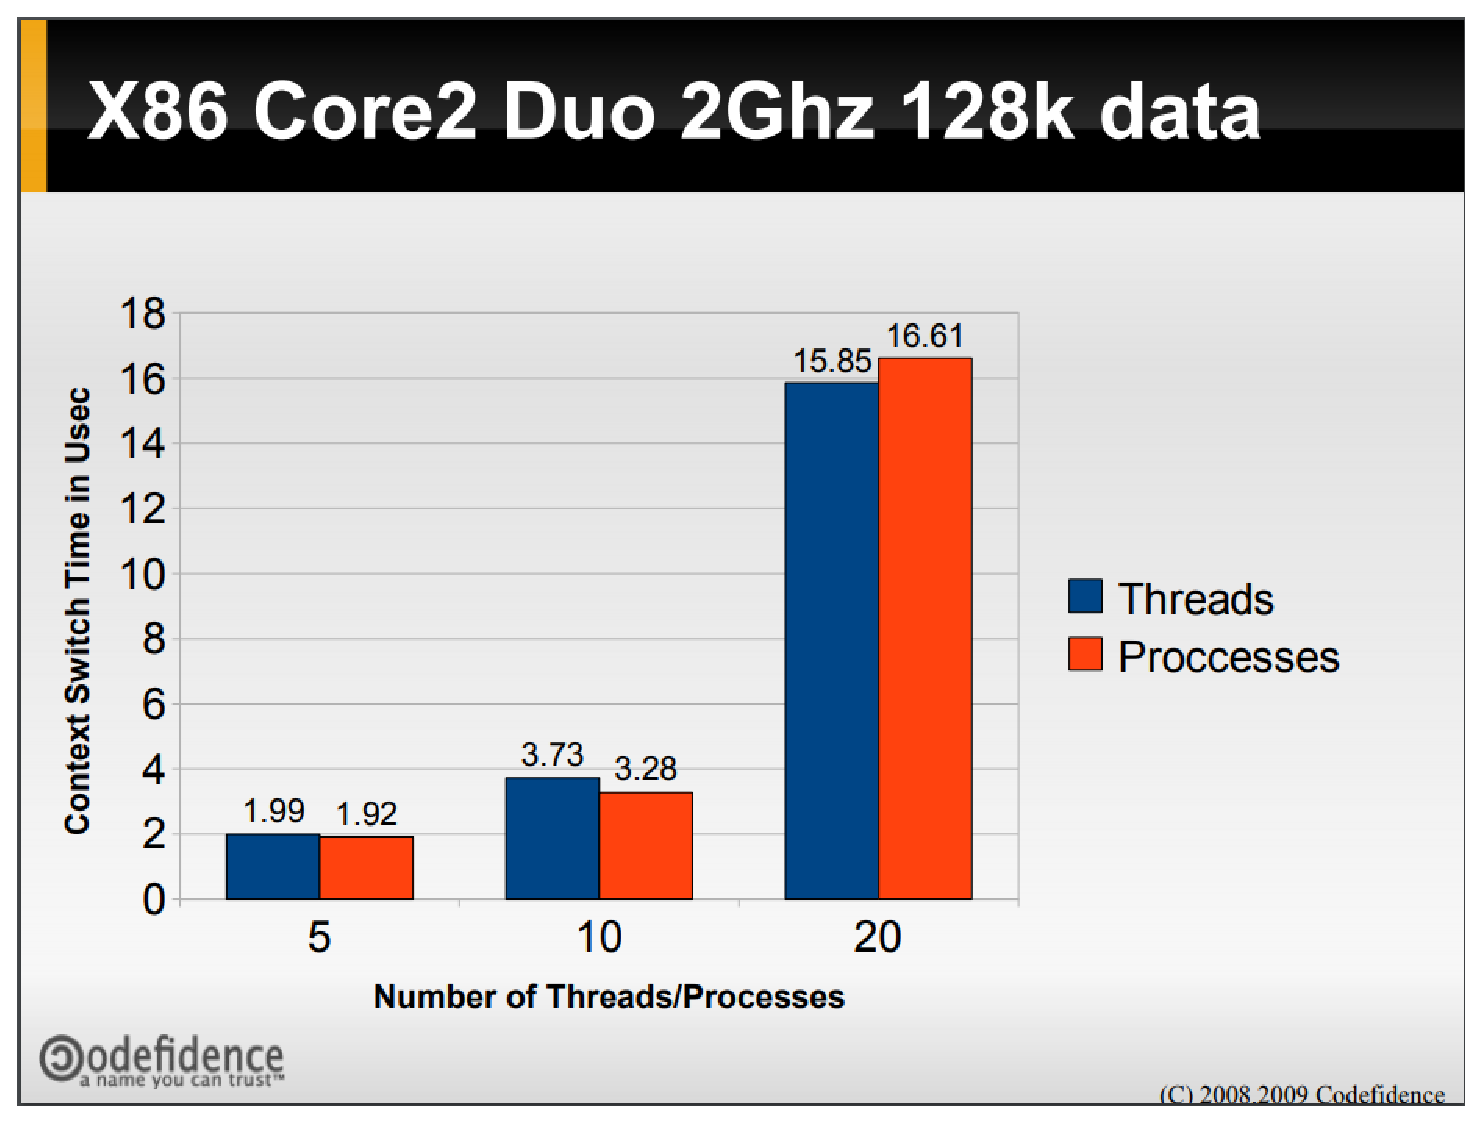
\includegraphics[width=0.6\textwidth]{context_switch_overhead.eps}
\captionof{figure}{Graph showing time it takes to context switch for both threads and processes on Linux \cite{LinuxSlides}}
\end{center}
\end{minipage}
\\ \\Thus, there is no strong case to be made from a performance perspective for why processes in Linux cannot handle the responsibilities often given to threads.

As for historical context, one must recall that early versions of the Linux kernel did not support multi-threading at all, treating such applications like any other normal process \cite{LinuxKernel}. Instead, the multiple lines of execution were handled and scheduled entirely in User Mode \cite{LinuxKernel}. When this old approach was deemed to be unsatisfactory as multi-threaded applications became the norm, Linux simply adapted their existing process structures to support multi-threaded applications with the use of lightweight processes.
\section{Scheduling}
As before, we will start with Windows. Windows utilizes a priority-driven, preemptive scheduling system \cite{WindowsInternals}. But since both FreeBSD and Linux also use schedulers that could be accurately described as being priority-driven and preemptive (in that if a higher priority thread is scheduled, the CPU context switches to it), we must dig deeper into the implementation details to uncover how these three schedulers differ. Although the functionality of the Windows scheduler, known more formally as the dispatcher, is spread throughout the kernel, it still behaves as a single entity, performing scheduling for all CPUs at all priority levels (excluding interrupts). Each thread has a priority composed of two parts: the base priority, which is a function of its process type, and the relative thread priority, which may change from thread to thread \cite{WindowsInternals}. Taken together, this priority is used to determine which threads get scheduled in what order. While a thread's base priority generally remains static, non-real-time threads can have their relative priorities changed based on a variety of system conditions. Threads of the same priority are then executed in a round-robin fashion, each running for a quanta (or time slice in POSIX terms) before giving up the CPU. 

In this sense it is similar to FreeBSD's scheduler with a few minor caveats. Firstly, soft real-time threads are handled by a completely separate queue in FreeBSD, whereas Windows simply differentiates the soft real-time threads and normal threads via their priority level \cite{FreeBSD}. Secondly, FreeBSD additionally has a third queue specifically for idle threads, which only run on the CPU if no soft real-time or normal threads are runnable. Finally, the FreeBSD scheduler, known as the timeshare scheduler, is inherently biased in favor of interactive processes. This is because the timeshare scheduler degrades a non-real-time thread's priority whenever it consumes its time slice (or quanta) and upgrades it whenever it is idle. This means interactive processes which exhibit short bursts of computation followed by long bouts of idleness are generally given higher priority than long-running background tasks.

On the other hand, Linux' default scheduler, known as the Completely Fair Scheduler, also aims to fairly distribute CPU time, but in a different way. The CFS keeps track of a metric known as virtual runtime for each process \cite{CFS}. In essence, the less time a process has been given at the CPU, the higher its priority. This is done in order to balance CPU usage in the long term, if not the short term. Additionally, the CFS is unique among these three in its concept of sleeper fairness, or the treatment of threads that are not currently runnable as being equivalent to those on the runqueue \cite{CFS}. In this way, when said threads do finally require the CPU, the get a 'fair share', so to speak. 

Despite these slight implementation details, all three systems approach the issue of scheduling in very similar ways. All three have a soft real-time scheduling option that is treated as having inherently higher priority than default scheduling and all three utilize a "fair" scheduler for normal threads, sharing CPU time between threads of the same priority roughly equally. The key difference, then, is how much control the operating systems give the end user over the scheduling. For Windows, the answer is not very much. There is only one scheduler available that handles scheduling for every thread and it cannot be changed by the end user. Additionally, Windows even imposes restrictions on how high one can set the priority of a user-level thread, specifically requiring specific permissions to assign threads soft real-time priority. Linux, on the other hand, has a multitude of schedulers that implement different algorithms available and allows the user to assign different schedulers to specific processes. If they don't like the ones provided, they are additionally free to extend them or even create their own. Naturally, since Windows is closed-source, extensibility of existing implementations is a non-option and the wider variety of scheduler options available out of the box for Linux reflects the wider variety of environments Linux is expected to run on (all kinds of servers, mobile devices, consoles, embedded systems, etc.)

\section{Conclusion}
In conclusion, although FreeBSD, Windows, and Linux, being operating systems, must all implement processes and scheduling in one way or another to accomplish the end goal of concurrency (perceived or otherwise), the details of said implementations vary greatly as a result of the history of these systems, the accessibility of their source code, and the hardware platforms they aim to run on.
\bibliographystyle{IEEEtran}
\bibliography{mybib}

\end{document}
